\documentclass[12pt, a4paper]{article}

\usepackage[utf8]{inputenc}
\usepackage[russian]{babel}
\parindent 0pt
\parskip 8pt
\usepackage{amsmath}
\usepackage{amssymb}
\usepackage{array}
\usepackage{floatrow}
\usepackage{float}
\usepackage[left=2.3cm, right=2.3cm, top=2.7cm, bottom=2.7cm, bindingoffset=0cm]{geometry} % headheight=0pt,
\usepackage{hyperref}
\usepackage{graphicx}
\usepackage{multicol}
\usepackage{fancyhdr} 
\usepackage{extramarks}
\usepackage[usenames,dvipsnames]{color}
\usepackage[normalem]{ulem}
\usepackage{titlesec}
\usepackage{tikz}
\definecolor{grey}{RGB}{128,128,128}

\pagestyle{fancy}
\fancyhf{}
\lhead{Билет № 1.6}
\chead{Носители информации: \\ магнитные, оптические и на основе флеш-памяти, RAID}
\rhead{\thepage}
\lfoot{made with gaporf}
\cfoot{}
\rfoot{\today}
\renewcommand\headrulewidth{0.4pt}
\renewcommand\footrulewidth{0.4pt}


\titlespacing*{\section}{0pt}{5pt}{0pt}
\titlespacing*{\subsection}{0pt}{5pt}{0pt}
\titlespacing*{\subsubsection}{0pt}{5pt}{0pt}

\begin{document}

\section{Магнитные накопители}

\subsection{Дискеты}

\begin{center}
{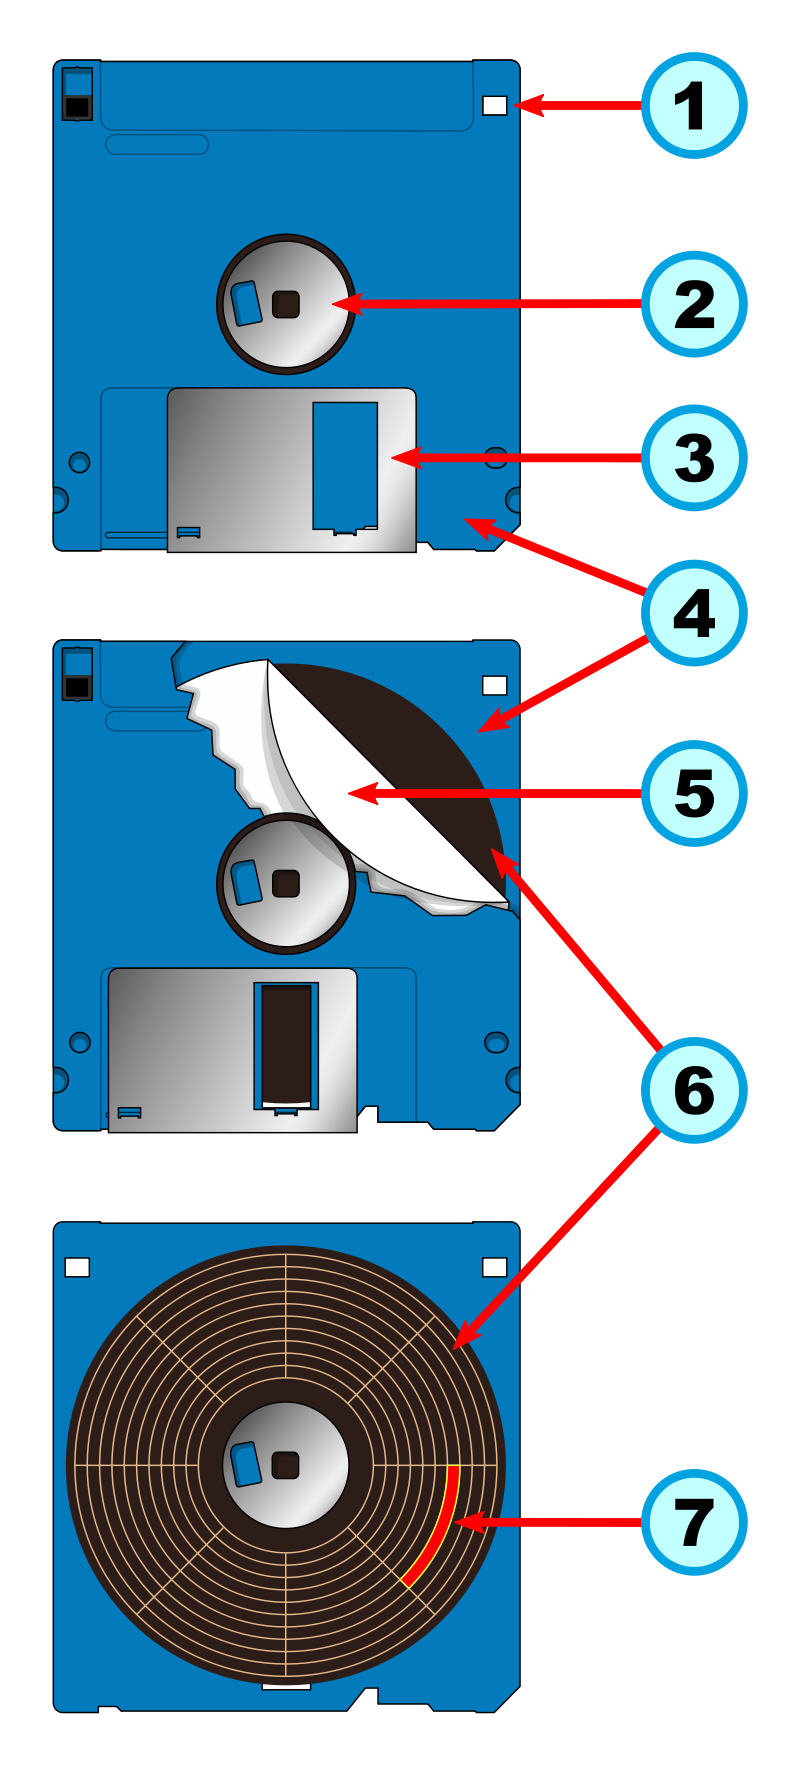
\includegraphics[scale=0.15]{./images/Floppy.png} \\ Устройство дискеты: 1) Информация об объёме дискеты. 2) Мотор, вращающий диск. 3) Затвор, предохраняющий диск от повреждения. 4) Пластиковая оболочка. 5) Полиэстер, предотвращающий трение диска. 6) Диск со специальным покрытием. 7) Сектор диска. }
\end{center}

Дискета представляет собой круглый диск, на который нанесено специальное покрытие, сохраняющее свойство намагниченности (информация на таких дисках хранится с помощью состояний магнитного поля). Есть специальная считывающая головка и маленькое отверстие, с помощью которого магнитная головка и считывает информацию с диска. Разные дискеты отличаются по возможности записи с двух сторон, количеством дорожек и секторов. В качестве примера рассмотрим дискету от Apple (\href{https://en.wikipedia.org/wiki/List_of_floppy_disk_formats}{вот тут красивая табличка}). В ней запись производится с двух сторон диска, всего имеется $80$ дорожек, и на каждой дорожке по $18$ секторов. Каждый сектор позволяется хранить $512$ байт полезной информации, итого общий объём равен $512 \cdot 18 \cdot 80 \cdot 2 = 1 \ 474 \ 560$ байт.

Каждый сектор на дискете задаётся с помощью CHS (Cylinder-head-sector), где первый параметр $C$ отвечает за номер дорожки, второй параметр $H$ - за сторону диска, а третий параметр $S$ - за номер сектора. 

Поскольку при высоких температурах диск расширяется, то головка, считывающая информацию, не всегда попадает на тот сектор, который нужен. Для этих целей в каждом секторе хранится служебная информация о том, какой номер дорожки и сектора. Помимо этого, требуется также гарантировать корректность данных. Для того, чтобы проверять корректность данных используют CRC (Cyclic redundancy check), или по-простому хеш-функцию. Каждый раз при записи на дискету или при чтении данных требуется считать хеш-функцию для полученных байтов и сверять её с CRC, если они совпадают, то мы, вроде бы, не проиграли (шанс коллизии очень мал). Но также используют коды коррекции ошибок ECC (Error correction code), которые позволяют исправлять неправильно записанные биты (более подробно можно почитать про коды Рида-Соломона, но суть такова, что если мы к нашим $N$ битам полезной информации дописываем $M$ битов этого кода, то можем с легкостью исправить $\frac{M}{2}$ битов среди получившихся $N+M$ битов). Заметим, что мы \textbf{вначале} считаем и записываем CRC, и только потом накладываем ECC.

Ещё стоит поговорить про сектора. На картинке видно, что сектора около центра и сектора на краю имеют разный размер, но объём информации хранят одинаковый. С этим придётся жить.

\subsection{Жесткий диск (HDD)}

\begin{center}
{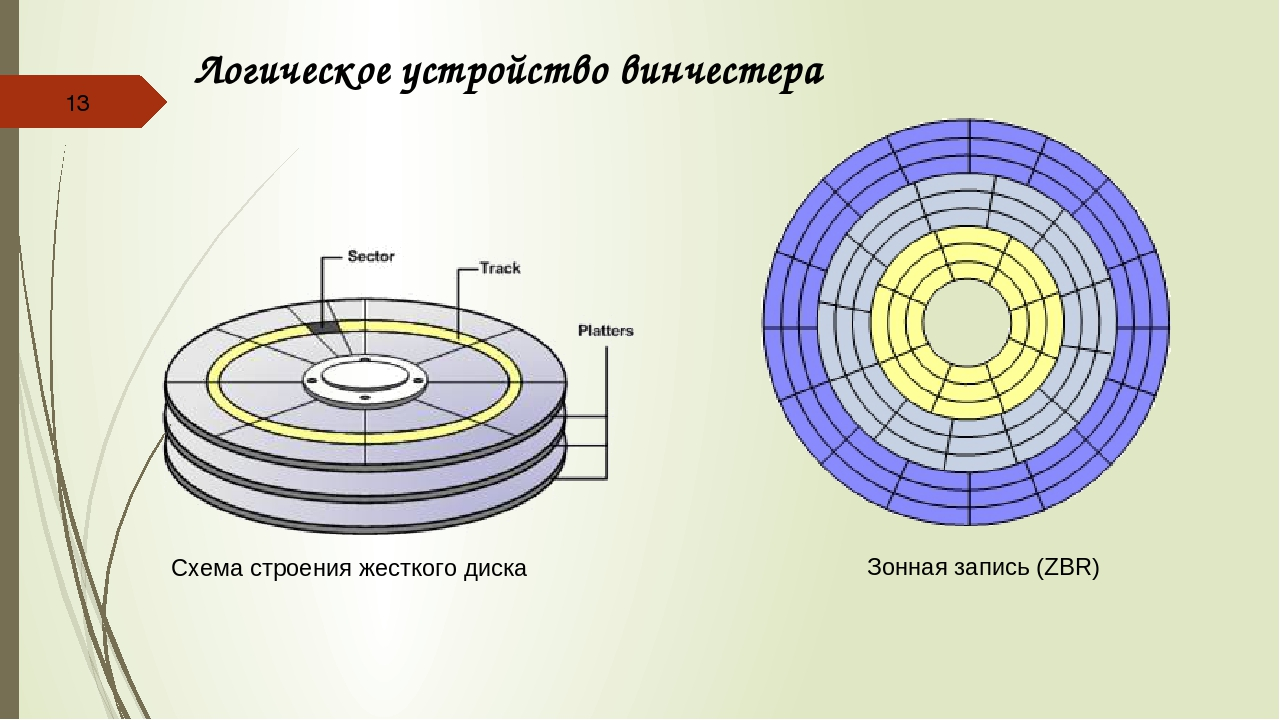
\includegraphics[scale=0.3]{./images/SectorsInHDD.jpg} \\ Сектора в HDD}
\end{center}

Как увеличить объём дискеты? Давайте жёстко закрепим диск, не будем давать хомячкам доступа к самому диску (в дискете это сделать могли), за счёт отсутствия грязи и пыли на диске можем записывать данные максимально плотно. Также разделим сектора нормальным (не как на дискете) образом. За счёт этого получили улучшенный вариант дискеты, который до сих пор используется в наших компьютерах.

Также теперь очевидно, что сектора располагаются произвольным образом, поэтому задавать сектора с помощью CHS стало немного неудобно. Отдадим эту задачу самому HDD, а мы будем считать, что у нас память линейна (старый чит). Назовём это LBA (Logical block addressing). Править ошибки будем аналогично дискете. 

Плюс в увеличении объёма сектора заключается в том, что при одинаковых затратах памяти на хранении CRC и ECC что, например, для восьми маленьких секторов, что для одного большого, состоящего из восьми маленьких шанс того, что мы не сможем восстановить данные у большого сектора ниже, чем хотя бы у одного из восьми маленьких (тут идёт банальная математика, ибо пусть для маленького сектора, состоящего из $N$ бит (полезных $+$ служебных), мы можем исправить только $k$ бит, то для большого сектора, состоящего из $8N$ бит мы можем исправить $8k$ бит, т.е. если в одном из маленьких секторов было запорото $k+1$ бит, то мы проиграли бы, в то время как при использовании большого сектора мы смогли бы исправить эти $k+1$ бит).

Но когда-то давно в качестве размера сектора для HDD был выбран размер в $512$ байт, и многие программы, грубо говоря, использовали это число как константу. По этой причине переход на $4$ КБ вызвал небольшие драмы, поскольку необходимо было как-то заточить HDD под те плохие программы. По этой причине диски, у которых размер сектора $4$ КБ могут как бы для системы читать по $512$ байт, но если программе нужно считать $4$ КБ, то мы проигрываем по всем параметрам, т.к. по $8$ раз читаем один и тот же сектор. 

\begin{center}
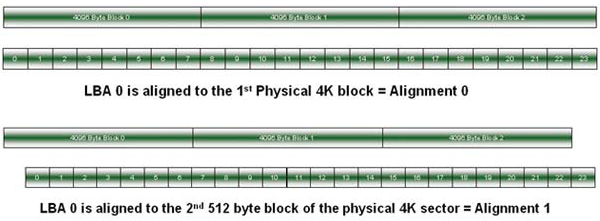
\includegraphics[scale=0.5]{./images/example.jpg}
\end{center}

Ещё есть такая штука, когда компьютер может работать только с секторами по $512$ байт, а HDD хранит секторы по $4$ КБ. Каждому маленькому сектору по $512$ байт присвоен уникальный номер из LBA. Аналогично и сектора в HDD имеют свои уникальные номера. И когда мы пытаемся сделать биекцию между номерами в ОС и номерами в HDD, то получается $8$ различных случаев, где начинается первый сектор. Это ситуация называется выравнивание, и если номер маленького сектора в ОС кратен $8$, то мы не совсем проиграли, в остальных случаях мы начнем терять немного скорости. Поэтому сейчас при использовании различных старых версий ОС рекомендуется начинать нумеровать сектора с номеров, кратным $8$. 

S.M.A.R.T. (Self-Monitoring, Analysis and Reporting Technology) - фича, которая позволяет отслеживать общее состояния диска и для каждого сектора выводит значение от $0$ до $100$, которое и говорит о том, насколько хорошо использовать этот сектор, а если всё плохо, то позволяет программно избегать использования этих секторов (вместо поврежденного сектора начинает использовать запасной, хотя ОС об этом даже и не узнает).

Производители хотят ещё увеличить плотность записи в HDD, поэтому пока есть следующие идеи:
\begin{enumerate}
	\item HAMR (Heat-assisted magnetic recording) - когда мы позволяем писать на жёсткий диск только в том случае, если он нагрет до определённой температуры: таким образом, мы можем ещё уплотнить данные, т.к. достаточно нагревать всего маленький кусочек, тогда как в соседние кусочки ничего не запишется, т.к. они не нагреты до определённой температуры. Очевидно, что диск не очень любит такие издевательства, поэтому число записей становится весьма конечным.
	\item MAMR (Microwave-assisted magnetic recording) - тоже какая-то технология, которая позволяет писать данные точнее, т.е. повышает плотность записи.
\end{enumerate}

Следует учитывать, что это только задумки, в магазине вы не найдёте диски с такими технологиями.

\section{Оптические накопители}

\begin{center}
{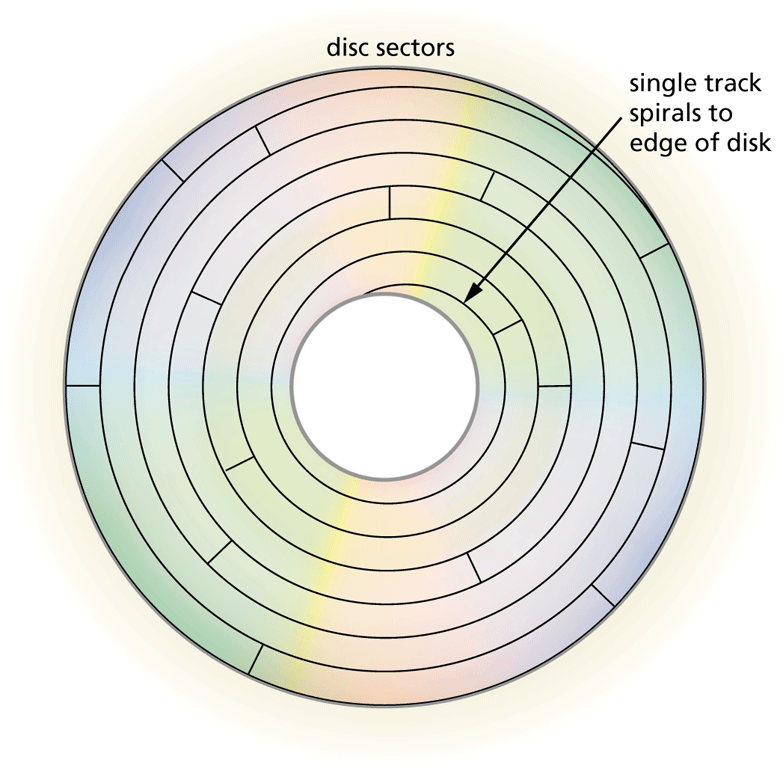
\includegraphics[scale=0.3]{./images/Optical.png} \\ Сектора в оптическом диске}
\end{center}

Оптические накопители являются наследниками виниловых пластинок, в них информация также хранится с помощью дорожек, на которых либо есть, либо нет ямок, и лазером проводится по диску, и в зависимости от того, как лазер отражается от дорожки, считывается информация. Запись диска производится за счёт лазера, который выжигает дорожки на специальном покрытии. Причём вполне себе возможно, что диски могут быть двухслойными, т.е. лазер с одной частотой считывает информацию с самого верхнего покрытия, потом меняет частоту и считывает информацию с нижнего покрытия.

Существует несколько поколений дисков: наиболее популярные CD (Compact disk) первого поколения, DVD (Digital video disc) второго поколения и Blu-ray третьего поколения. Также каждый диск может иметь разные плюшки, например CD-RW - позволяет переписывать диск несколько раз за счёт того, что диск нагревается, и сама поверхность расплавляется и все ямки разравниваются. Поскольку типов дисков очень много, то советую в википедии посмотреть типы ради общего развития.
   
Размер стандартного сектора составляет $2$ КБ полезных данных плюс несколько байт на служебную информацию. Также сделали финт с Audio CD: поскольку не так страшно, если несколько бит исказятся (человеческое ухо даже не услышит этого), то вместо служебной информации всё место в секторе отдано под полезную ифнормацию, таким образом мы получили размер сектор в $2 \ 352$ байта, но также были введены требования к звуку, а именно: стерео (двухканальная запись), $16$-битное кодирование звука, частота $44 \ 100$ Гц.

\section{Флеш-накопители}

\begin{center}
{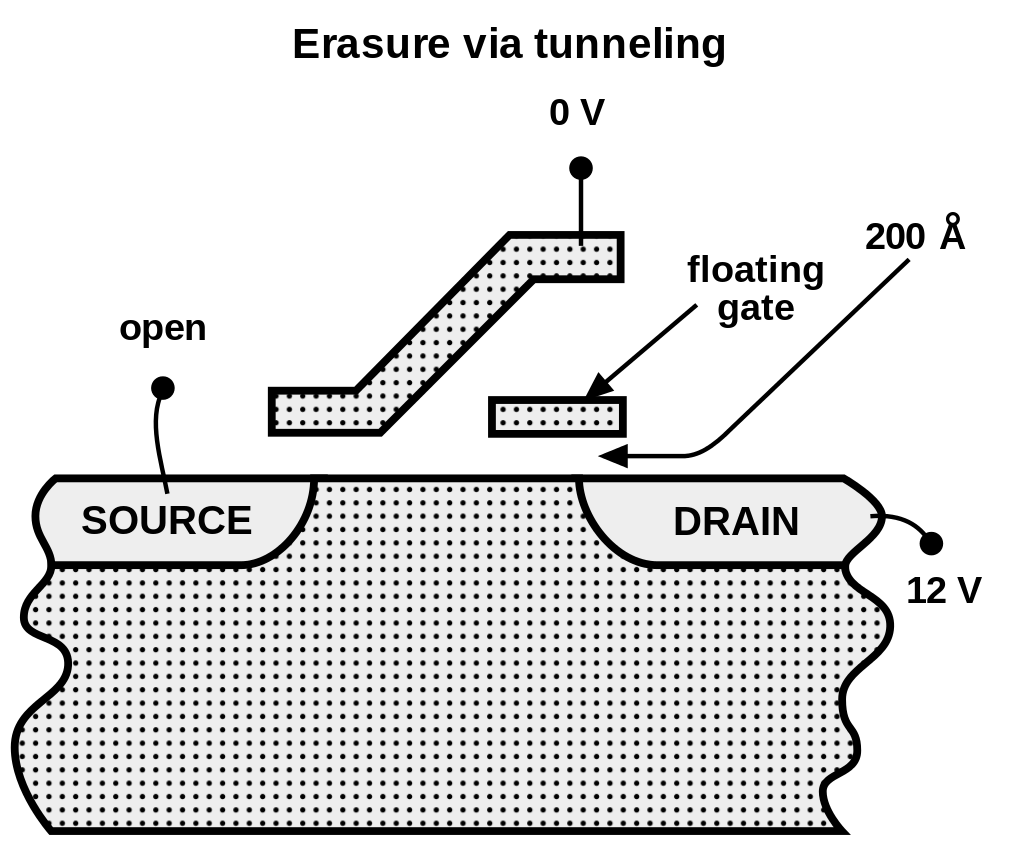
\includegraphics[scale=0.3]{./images/Flash_erase.png} \\ Схема транзистора с плавающим затвором, с помощью которого и кодируется информация во флеш-памяти}
\end{center}


Посмотрим на устройство RAM и поймём, что недостаток хранения данных с помощью транзисторов в том, что при отсутствии напряжения мы теряем данные. Для того, чтобы немного пофиксить этот недостаток возьмём транзисторы с плавающим затвором, суть которого заключается в том, что если подать напряжение на плавающий затвор, то мы <<заселим>> электроны, а если на подложку - то <<выселим>>. Сильным минусом таких транзисторов является то, что при перезаписи данных транзисторы деградирует, поэтому со временем мы будем получать не те состояния, которые в них записали. Существует следующие типы транзисторов:

\begin{enumerate}
	\item SLC (Single-level cell) - каждый транзистор хранит два состояния, $0$ и $1$. Очевидно, что <<подать мало напряжения и подать много напряжения реализовать проще всего>>, поэтому мы можем совершать до $100 \ 000$ операций перезаписей, а также записываем достаточно быстро, поэтому производители не очень любят SLC, поэтому флешки и SSD с такими типами транзистора не сыщешь в магазинах (хотя в SSD \textit{just for lulz} могут добавить небольшой модуль память на SLC, чтобы казалось, что память быстрая, и хомячки купили её);
	\item MLC (Multi-level cell) - каждый транзистор хранит четыре состояния - $0$, $1$, $2$ и $3$. Количество операций перезаписей уже $5 \ 000$, что сильно нас радует, а также данные записываются дольше (тут уже надо точнее подавать ток);
	\item TLC (Triple-level cell) - каждый транзистор хранит $8$ состояний, количество операций перезаписи уже $3 \ 000$, зато места занимает меньше, а записываются данные дольше;
	\item QLC (Quad-level cell) - каждый транзистор хранит $16$ состояний, количество операций перезаписи уже $1 \ 000$ (но Скаков говорил о нескольких десятках, но данный вид транзисторов ещё не шибко используется);
\end{enumerate}

Скорее всего, вы встретите или MLC, или TLC транзисторы в вашей флешке. Также, как это не звучало странно, SSD - флешка, но с умным контролером памяти и прочими кошерными вещами. 

Как бы это не было прискорбно, но флешки имеют маленький ресурс, а также производитель даёт гарантию, что если флешку не вставлять в компьютер, то информация \textbf{гарантированно} будет хранится не больше нескольких месяцев, а дальше как повезёт. Аналогично ситуация касается и SSD, но у них, вроде бы, всё получше, ибо есть умный контроллер памяти, который старается использовать транзисторы равномерно, в отличии от флешки, где пользователь сам дурак, если пишет в одно место $12 \ 345$ раз. а другие транзисторы вообще не использует. Такая же ситуация и со скоростью доступа/записи, поскольку флешка передают информацию довольно медленно. Чтобы покупали SSD, а не топовые HDD, у которых информация может хранится годами, а также количество перезаписей стремится к бесконечности, то в SSD делают несколько параллельных флеш-накопителей, а также стараются, по возможности, не сразу удалять все данные, а делать стирания тогда, когда к диску никто не обращается. И благодаря таким махинациям мы получаем выигрыш в скорости при использовании SSD, т.к. увеличить скорость у HDD не имеем возможности. 

Насчёт стираний. В HDD мы можем спокойно перезаписывать данные, поэтому нет необходимости в том, чтобы диск стирать (мы просто отмечаем, что место свободно и всё). В SSD просто так взять и записать данные поверх старых нельзя. Для этого придётся вначале применить операцию стирания блока, и уже на чистый блок записывать данные. Очевидно, что в этом случае мы будем записывать данные на чистый SSD быстрее, чем на полный. Поэтому и нужна операция $trim$, которая как бы стирает данные в тот момент, когда к диску никто не обращается, тем самым пытаясь повысить скорости записи в будущем. Ну и в HDD эта операция была введена для того, чтобы интерфейсы у HDD и SSD совпадали и не было никаких различий на уровне системы, какой именно диск стоит.

Интерфейсы у HDD и SSD совпадают, поэтому всё, что касается блоков в HDD применимо и к SSD.

\section{RAID}

\begin{flushright}
{\textit{Зайка требует, чтобы \\ мы знали RAID-0, RAID-1, \\ RAID-10, RAID-5, RAID-6}}
\end{flushright}

RAID (Redundant Array of Independent Disks) - технология, которая использует лишние диски для того, чтобы повысить производительности или безопасность данных. Существует несколько типов, но мы рассмотрим только те, которые требует Скаков.

\begin{center}
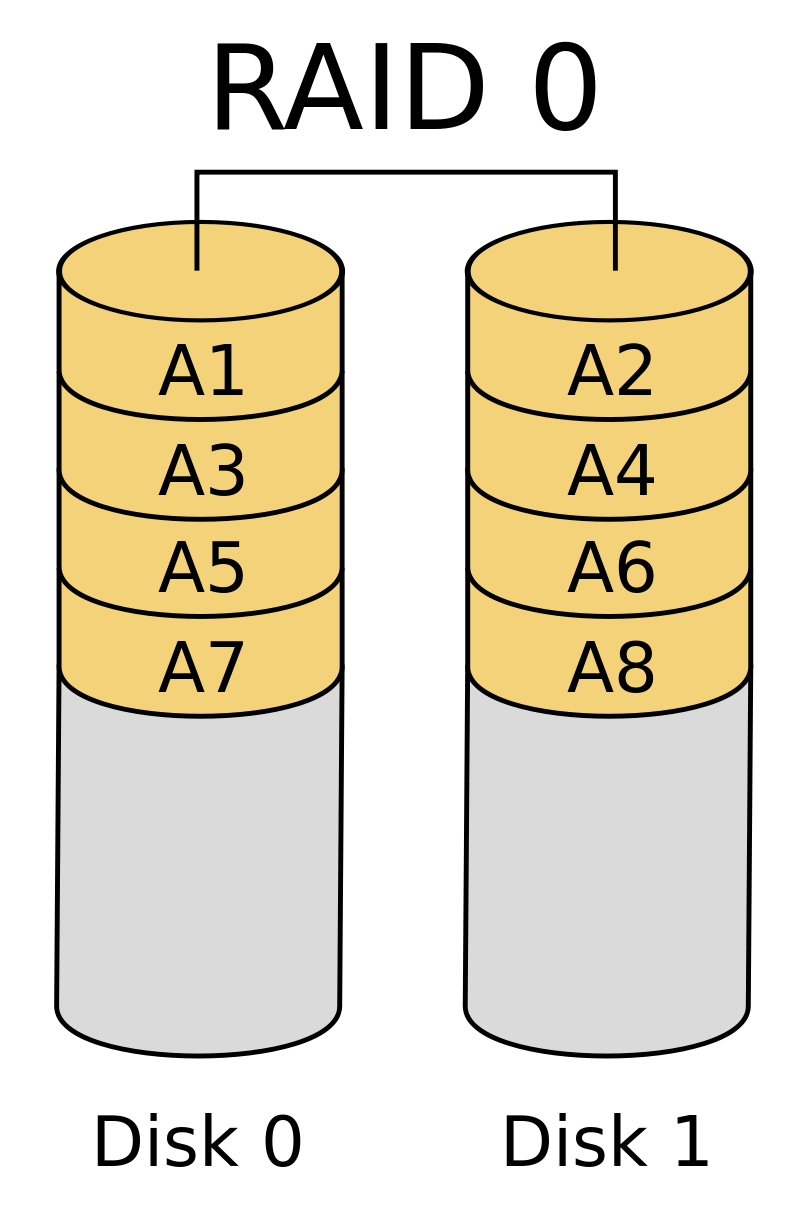
\includegraphics[scale=0.1]{./images/RAID0.png}
\end{center}

В этом случае мы просто разбиваем данные пополам, т.е. все блоки с нечетными номерами идут в первый диск, с чётными - во второй. Обобщается на случай, если у нас не $2$, а $n$ дисков. Очевидный профит в том, что мы можем читать наши данные в $n$ раз быстрее. Минус - если выйдет из строя хотя бы один сектор в одном из диске, то мы проиграем, т.е. нам нужно, чтобы оба диска не выходили из строя, но теория вероятностей говорит о том, что шанс того, что оба диска останутся в живых ниже, чем один.

\begin{center}
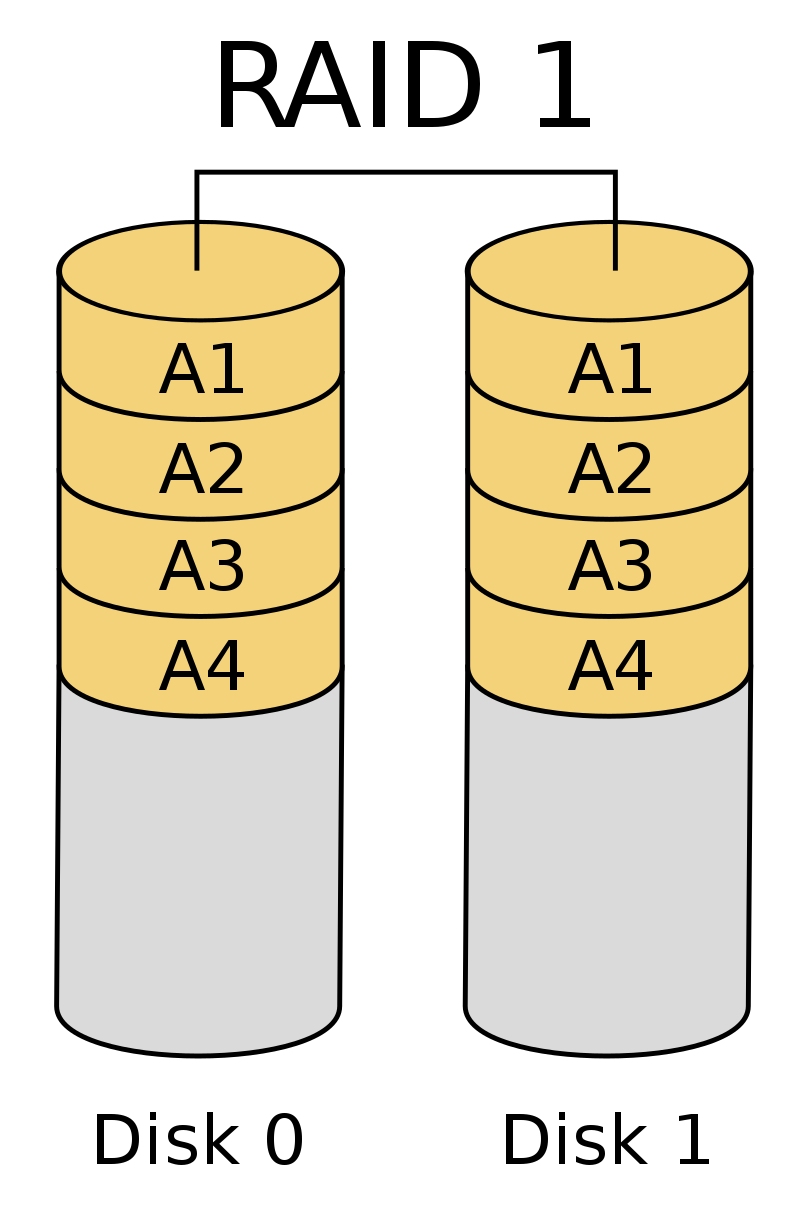
\includegraphics[scale=0.1]{./images/RAID1.png}
\end{center}

RAID 1 предлагает использовать два диска, чтобы хранить одну и ту же информацию. Таким образом мы можем ускорить чтение данных с диска, а также если сломается один из дисков, то спокойно можем использовать другой диск, т.е. повышаем надёжность такого источника хранения информации. Но главным минусов является то, что мы вынуждены использовать диски с объёмом в $2$ раза больше, чем храним реальной информации. Аналогично обобщается на случай $n$ дисков.

\begin{center}
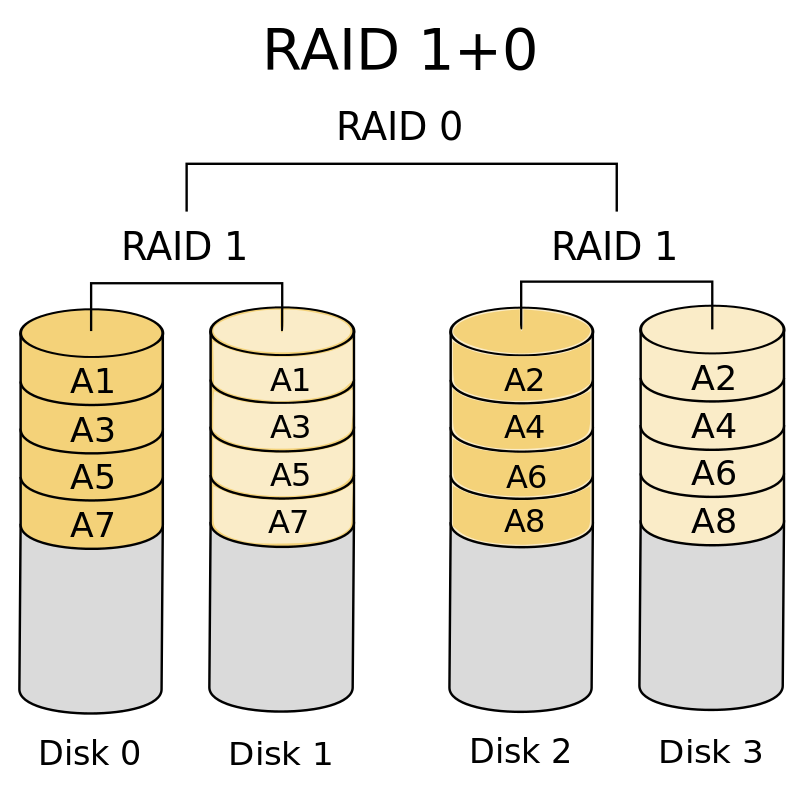
\includegraphics[scale=0.2]{./images/RAID10.png}
\end{center}

Возьмём и объединим RAID 1 и RAID 0, причем мы вначале делим данные на две части, и потом к каждой из части применяем операцию дублирования. 

\begin{center}
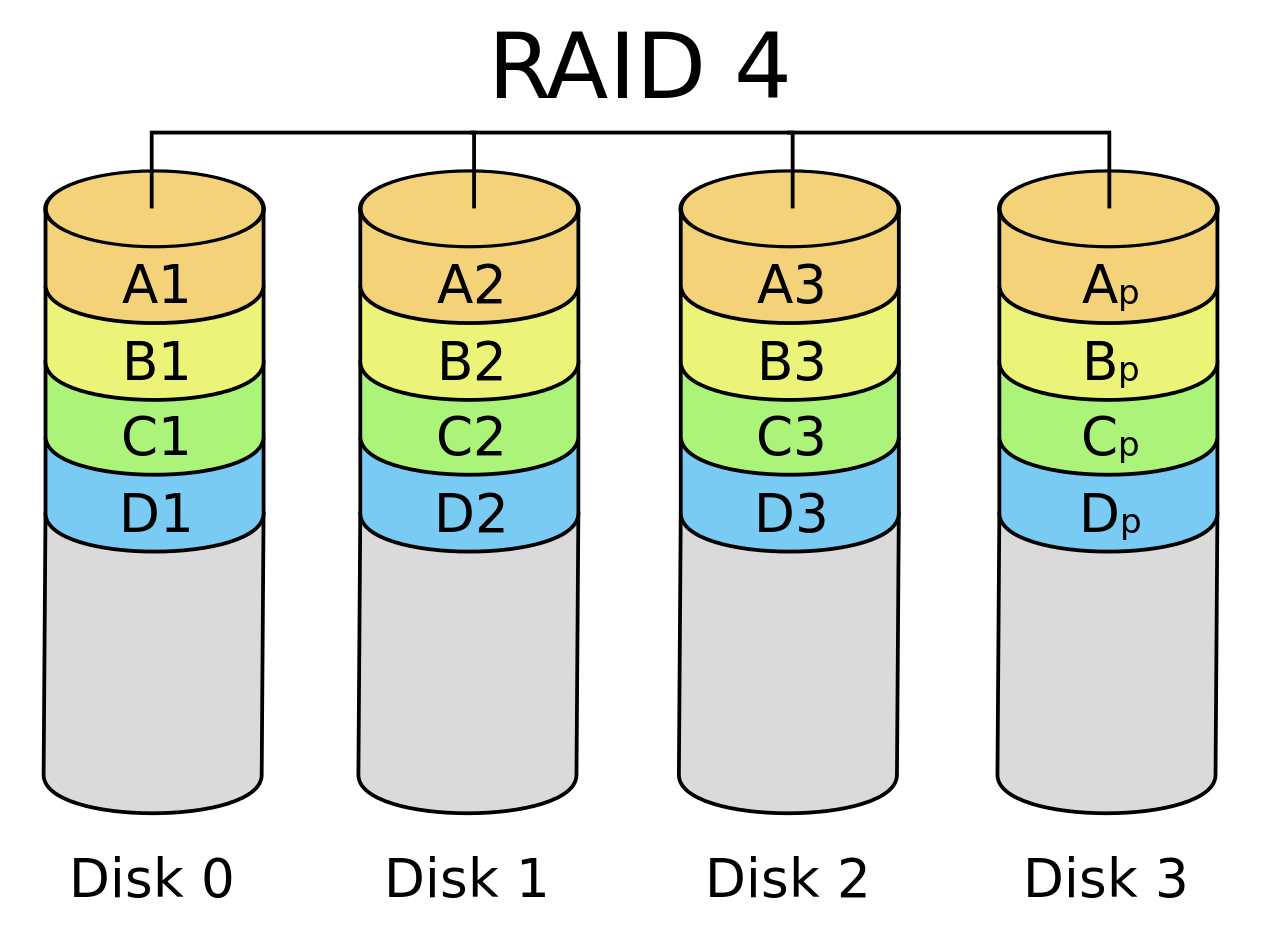
\includegraphics[scale=0.13]{./images/RAID4.png}
\end{center}

Пусть мы храним данные на $n-1$ дисках, тогда $n$-ый диск отдадим под хранения ксоров всех бит в соответствующих позициях битов (нормальные люди это называют битом чётности). Даёт довольно большой плюс, если нам надо читать данные с рандомных мест, но при записи очень сильно замедляется, поскольку надо постоянно переписывать последний диск. Данная конструкция довольно неплохо исправляет ошибки, если полетел один из дисков и не требует так много места, как RAID 1.

\begin{center}
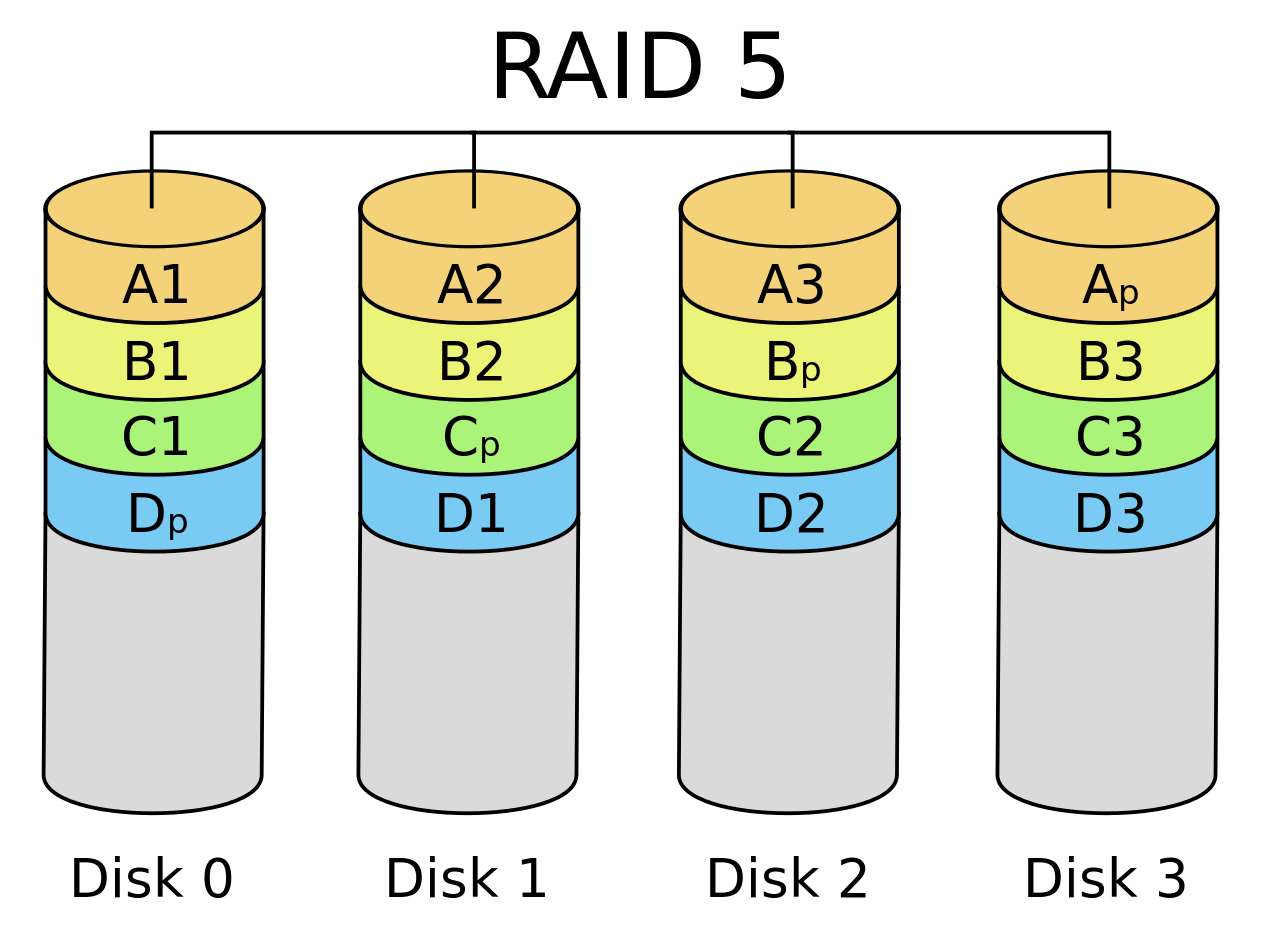
\includegraphics[scale=0.13]{./images/RAID5.png}
\end{center}

Распределим по всем дискам специальный сектор, ответственный за бит чётности. Теперь нам не надо каждый раз при записи данных на какой-то диск дёргать последний, а лишь соседний. При записи это даёт больше параллельности, чем RAID $4$.

\begin{center}
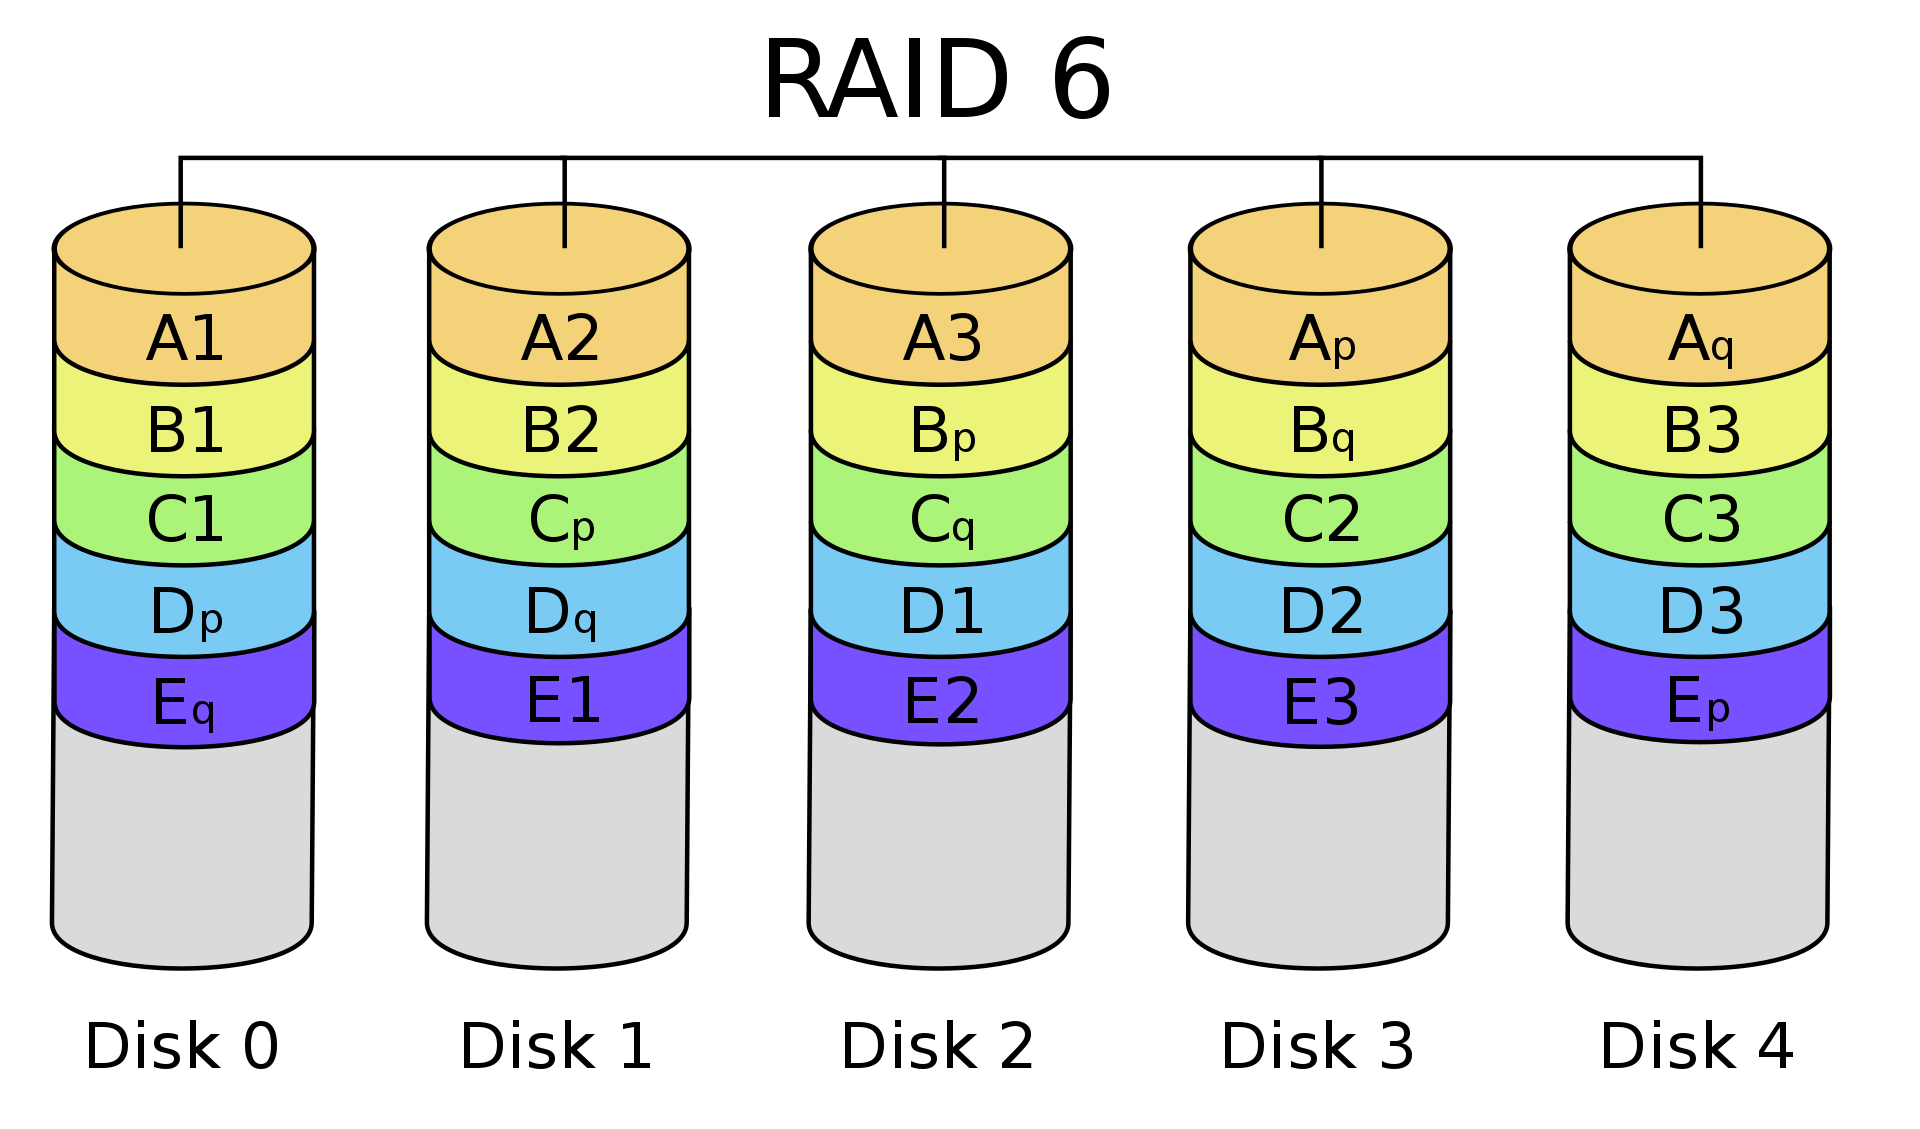
\includegraphics[scale=0.11]{./images/RAID6.png}
\end{center}

Теперь не один, а два блока используется для хранения и кода Рида-Соломона и ксора всех бит. Позволяет лучше исправлять ошибки, т.е. повышаёт надежность всего массива этих дисков. И параллельность позволяет делать какую-никакую.

\end{document}
